\subsubsection{Blazemark}
Blazemark is a benchmark suite provided by Blaze to compare the performance of Blaze with other linear algebra libraries. 

\subsection{Method}

	
\subsection{Experiments}
In order to capture the relationship between number of cores, \textit{chunk\textunderscore{size}}, \textit{block\textunderscore{size}}, and the performance, we ran a series of experiments with different of these parameters and measured the number of floating point operations per second performed. 

For these experiments ,at the first step we selected the $DMatDMatADD$ benchmark which was implemented in Blazemark. $DMatDMatADD$ benchmark is a level 3 BLAS function to perform matrix-matrix addition in the form of $A=B+C$, where $A$, $B$, $C$ are square matrices of the same size. 

To avoid adding the scheduling overhead for small matrix sizes, Blaze uses a threshold to start parallelization, which is specific to the type of operation. For matrix-matrix addition, if the number of elements in the matrix is greater than 36100 elements(which is equivalent to a square matrix of size 190 by 190) Blaze uses the configured backend to parallelize the assignment operation. For this reason, we start our experiments with matrix size of 200x200 and gradually increase the size to 1587x1587. 


Figure~\ref{fig1} shows the results of running $DMatDMatADD$ benchmark for matrix sizes and number of cores listed in \tablename{name} based on grain size. Grain size 

\begin{figure}[H]
	\centering
	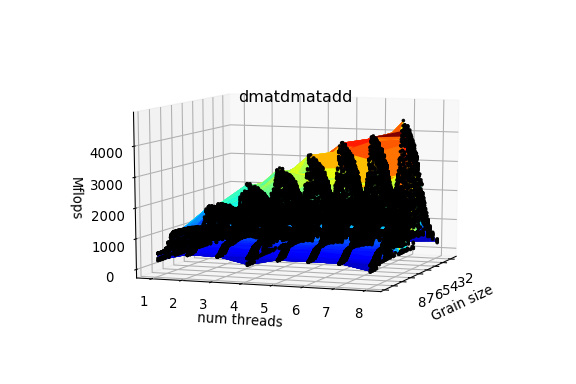
\includegraphics[width=1\linewidth]{images/fig1.png}
	\caption{An example of results obtained from Blazemark}	
	\label{fig1}
\end{figure}

\subsection{Observation}

\subsection{L2 cache miss analysis}
In this set of experiments we used the performance counters integrated into HPX to measure the cache miss rate for different grain\textunderscore sizes w

-grain\textunderscore size
